\section{Chameleon Gravity}
\label{sec_cham}
If there is a scalar field coupled to a non-relativistic matter with the interaction as strong as gravity, the coupling must be tuned to a small value to satisfy tests of the equivalence principle in Solar System which exclude any fifth forces. However, this fine-tunning can be avoided and the coupling can be of order of unity with the so called \textit{chameleon mechanism}.

The action of a chameleon scalar field $\phi$ is given by the action \eqref{eq:S_ein_fr} in the Einstein frame
\eq{
	\label{cham}
	S=\int\dd^4x\dg\left[\frac{\Mpl^2}{2}R - \frac12(\partial\phi)^2-V(\phi)\right]+S_m[\psi_m^{(i)};g_\uv^{(i)}].
}
It is the same action as for the normal quintessence but now the matter fields are coupled to a metric $g_\uv^{(i)}$, which is related to the Einstein frame metric $g_\uv$ by a conformal transformation
\eq{
	\label{cnf_cpl}
	g_\uv^{(i)}=e^{2\beta_i\phi/\Mpl}g_\uv.
}
Varying the action \eqref{cham} with respect to the field $\phi$ one can obtain the equation of motion
\eq{
	\label{eom:cham}
	\Box\phi=V_{,\phi}-\sum_i\frac{\beta_i}{\Mpl}e^{4\beta_i\phi/\Mpl}g^\uv_{(i)}T^{(i)}_\uv,
}
where
\eq{
	T^{(i)}_\uv\equiv\frac{-2}{\dg}\frac{\delta(\dg\LL_m)}{\delta g^\uv_{(i)}}
}
is the stress-energy tensor for the $i$-th matter component. Note that the stress-energy tensor defined in this way is \textbf{not} conserved in the Einstein frame, but rather in the Jordan frame, i.e.
\eq{
	\tilde{\nabla}_\mu T_{(i)}^\uv=0,
}
where $\tilde{\nabla}_\mu$ is the covariant derivative corresponding to the Jordan frame metric and we are assuming that the individual matter species do not interact with each other. The trace (not a scalar in the Einstein frame) of the $i$-th component is defined as $T^{(i)}\equiv g^\uv_{(i)}T^{(i)}_\uv$. For a perfect isentropic fluid is $T^{(i)}=-(1-3w_i)\tilde{\rho}_i$ with $\tilde{\rho}_i$ the energy density in the Jordan frame. The energy density defined as
\eq{
	\rho_i\equiv\tilde{\rho}_ie^{3(1+w_i)\beta_i\phi/\Mpl},
}
is conserved in the Einstein frame \parencite{Waterhouse:2006wv}.

Equation of motion \eqref{eom:cham} is then
\eq{
	\Box\phi=V_{,\phi}+\sum_i(1-3w_i)\frac{\beta_i}{\Mpl}\rho_i e^{(1-3w_i)\beta_i\phi/\Mpl}.
}
This equation could be read as
\eq{
	\Box\phi=V_{\eff,\phi}\left(\phi\right),
}
where the effective potential $V_{\eff}$ is defined by
\eq{
	V_{\eff}\left(\phi\right)\equiv V(\phi)+\sum_i\rho_i e^{(1-3w_i)\beta_i\phi/\Mpl}.
}
If the couplings $\beta_i$ are the same for each matter component with the same $w$ (we can omit the radiation in the sum) and the overall density is $\rho=\sum_i\rho_i$, then the effective potential reads
\eq{
	V_{\eff}\left(\phi\right)\equiv V(\phi)+\rho e^{(1-3w)\beta\phi/\Mpl}.
}
For the quasi-static and weak $(\beta\phi/\Mpl\ll1)$ field in a weak gravity background (the Minkowski background) with non-relativistic matter, the equation further simplifies as
\eq{
	\label{eq:cham}
	\Delta \phi=\frac{\beta}{\Mpl}\rho+V_{,\phi},
}
which looks like the normal Poisson equation but with an extra non-linear term.
\subsection{Chameleon Force}
The interaction of the chameleon field with matter is described by the conformal coupling \eqref{cnf_cpl}. As the matter fields $\psi_m^{(i)}$ couple to the metric $g_\uv^{(i)}$ instead of $g_\uv$, free test particles follow geodesics of $g_\uv^{(i)}$
\eq{
\frac{\dd^2x^\mu}{\dd\tilde{\tau}^2}+\tilde{\Gamma}^\mu_{\alpha\beta}\dddd{x^\alpha}{\tilde{\tau}}\dddd{x^\beta}{\tilde{\tau}}=0,
}
where $\tilde{\Gamma}^\mu_{\alpha\beta}$ are the Christoffel symbols of the metric $g_\uv^{(i)}$. In the Einstein frame metric this gives \parencite{Waterhouse:2006wv}
\eq{
\frac{\dd^2x^\mu}{\dd\tau^2}+\Gamma^\mu_{\alpha\beta}\dddd{x^\alpha}{\tau}\dddd{x^\beta}{\tau}=-\frac{\beta_i}{\Mpl}\left(2\phi_{,\alpha}\dddd{x^\alpha}{\tau}\dddd{x^\mu}{\tau}+g^{\beta\mu}\phi_{,\beta}\right).
}
Note that the chameleon force violates the weak Equivalence Principle only if there exist two matter species with differing values of $\beta_i$. In the non-relativistic limit, a test particle of mass $m$ of species $i$ in a static chameleon field $\phi$ is moving under a force $\vec{F}_\phi$ given by
\eq{
\label{cham_force}
\frac{\vec{F}_\phi}{m}=-\frac{\beta_i}{\Mpl}\vec{\nabla}\phi
}
\subsection{Chameleon mechanism}
As discussed in \autoref{screen} we need some sort of a screening mechanism to avoid Solar System tests of GR. It means as seen from \eqref{cham_force} that the chameleon potential needs to approach some constant value in dense regions.

Suppose we have a background solution $\phi_\infty$ which minimizes the effective potential with $\rho=\rho_\infty$. For small fluctuations $\phi=\phi_\infty+\delta\phi$ and $\rho=\rho_\infty+\delta\rho$ we can linearized \eqref{eq:cham} to obain
\eq{
\label{eq:cham_lin}
\Delta \delta\phi=\frac{\beta}{\Mpl}\delta\rho+m^2_\infty\delta\phi,
}
where
\eq{
m^2_\infty\equiv V_{,\phi\phi}(\phi_\infty).
}
Except for the screening term, which often could be neglected, the equation \eqref{eq:cham_lin} has the same behavior as the Poisson equation for the Newtonian potential $\Phi_N$. For a spherically symmetric density profile this gives solution
\eq{
\phi=\phi_\infty+2\beta\Mpl\Phi_N\left(r\right)e^{-m_\infty r}.
}
As the objects in the background become more massive (larger and/or denser) the Newtonian potential grows larger (in magnitude) and so the deviation of $\phi$ from background solution $\phi_\infty$. At some point this deviation is no longer small and the potential term in \eqref{eq:cham} cannot be treated perturbatively. It starts canceling the first source term and eventually the field $\phi$ posses a new (constant) value which minimizes the effective potential inside an object.

This is the essence of the chameleon mechanism. Let us derive the mechanism in a more proper and exact way.
\subsection{Chameleon Profile}
\label{cham_prof}
To obtain the cosmic acceleration and chameleon behavior described above we need to choose a chameleon potential $V(\phi)$ with the right properties. As in the case of the quintessence field we need the slow-roll mechanism to provide the acceleration and therefore we need the potential where the field rolls down in a potential slope. To have a screening mechanism in \eqref{eq:cham} we need $V_{,\phi}<0$ and so field rolls down in the positive direction. And finally to have a screening behavior of the field as in  the case of the Yukawa potential we need a real mass of the field, i.e. $V_{,\phi\phi}>0$.

These properties of the potential are commonly referred to as the potential of the \textit{runaway} form:
\begin{enumerate}
	\item $\lim_{\phi \to 0}V\left(\phi\right)=\infty$;
	\item $V\left(\phi\right)$ is $C^\infty$, bounded below;
	\item $V_{,\phi}<0$ and increasing;
	\item $V_{,\phi\phi}>0$ and decreasing.
\end{enumerate}
Although the item $1.$ and boundedness from $2.$ are usually assumed as these kinds of potentials arise in in supersymmetric models, there are not necessary as we will see in the \autoref{sec:num_cham} where we will study the chameleon gravity in context of Hu-Sawicki $f(R)$ models.

Example of this runaway potential we have already seen in the quintessence models -- the inverse power-law potential \eqref{Qtr}
\eq{
V(\phi)=M^{4+n}\phi^{-n}\ (n>0).
}
Another example is the exponential potential
\eq{
V(\phi)=M^4\exp{\frac{M^n}{\phi^n}}\ (n>0).
}
We wish to find a solution for spherically symmetric matter distributions of a single species of pressureless matter such that
\begin{equation*}
\rho(r)=
\begin{cases}
\rho_c & r<R_c \\
\rho_\infty & r>R_c,
\end{cases}
\end{equation*}
where $\rho_c>\rho_\infty$. Further we define $\phi_c$ and $\phi_\infty$ with their masses $m_c$ and $m_\infty$ (the masses of small fluctuations about $\phi_c$ and $\phi_\infty$) such as
\begin{align*}
V_{\eff,\phi}\left(\phi_c\right)_{|\rho=\rho_c}&\equiv0	&	m^2_c&\equiv V_{\eff,\phi\phi}\left(\phi_c\right) \\
V_{\eff,\phi}\left(\phi_\infty\right)_{|\rho=\rho_\infty}&\equiv0	&	m^2_{\infty}&\equiv V_{\eff,\phi\phi}\left(\phi_\infty\right).
\end{align*}
The effective chameleon potential for this configuration is shown in \autoref{fig_eff_pot}. In the background with low density, the curvature of the potential is much shallower, corresponding to a light scalar that mediates a long range force. Inside the object of high density, the scalar acquires a large mass, and the force shuts off.
\begin{figure}
	\centering
		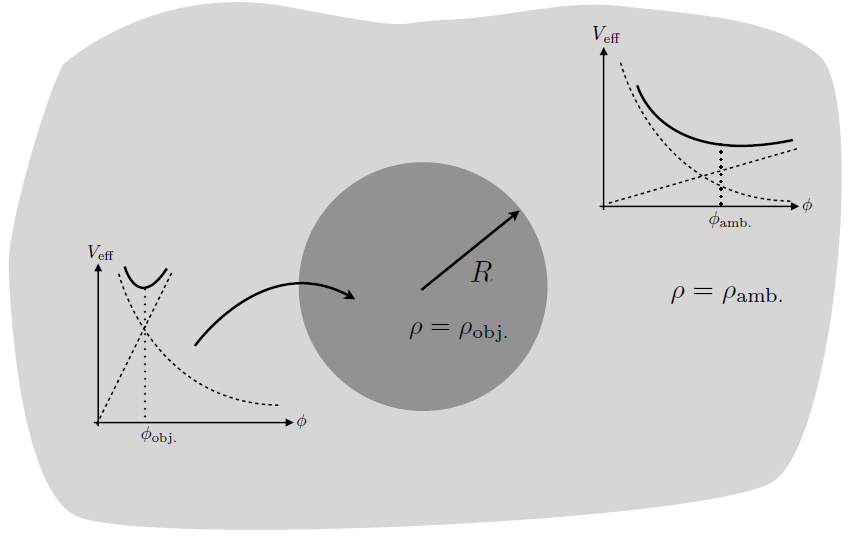
\includegraphics[scale=0.70]{modif_grav/eff_pot.png}
	\caption{The effective chameleon potential for a massive spherical object of density $\rho_{\mbox{\scriptsize{obj.}}}$ surrounded by the background with density $\rho_{\mbox{\scriptsize{amb.}}}$. From \textcite{2015PhR...568....1J}.}
	\label{fig_eff_pot}
\end{figure}

In spherical coordinates assuming spherical symmetry, equation \eqref{eq:cham} becomes
\eq{
\label{eq_cham_r}
\frac{\dd^2\phi}{\dd r^2}+\frac{2}{r}\dddd{\phi}{r}=\frac{1}{r}\frac{\dd^2\left(r\phi\right)}{\dd r^2}=V_{,\phi}\left(\phi(r)\right)+\frac{\beta}{\Mpl}\rho(r).
}
We must impose two boundary conditions which are
\begin{align*}
\dddd{\phi}{r}(r=0)&=0 \\
\phi(r\rightarrow\infty)&=\phi_\infty.
\end{align*}
The first one corresponds to a non-singularity of the solution at the origin while the later one ensures that the chameleon force vanishes at the infinity (as $\dd\phi/\dd r\rightarrow0$).

The equation \eqref{eq_cham_r} drives the field $\phi$ toward the $\phi_\infty$ outside the object and toward $\phi_c$ inside the object. Note that the second term acts like the friction term.

In order to solve \eqref{eq_cham_r} we must do several approximations. Outside the object we assume that the field sits near the extreme $\phi_\infty$ and we can linearized our equation
\eq{
\frac{1}{r}\frac{\dd^2\left(r\phi\right)}{\dd r^2}=m^2_\infty(\phi-\phi_\infty),
}
with the decaying solution
\eq{
\phi(r)=-\frac{\beta}{4\pi\Mpl}\frac{\tilde{M}}{r}e^{-m_\infty r}+\phi_\infty.
}
Note that the integration constant $\tilde{M}$ is not generally the mass of the object $M_c$ as in the case of the Newtonian potential because it is determined by the field inside the object which has different behavior than the Newtonian potential. As we will see later, for small Newtonian potentials (in magnitude) this effective mass $\tilde{M}\approx M_c$ but as the potential grows larger part of the object`s mass is screened away $\tilde{M}< M_c$.

Inside the object we use one of the two approximations based on the initial value of $\phi_i\equiv\phi(0)$ -- either $\phi_i\approx\phi_c$ or $\phi_i\gg\phi_c$ .
\subsubsection{Thin-shell regime}
In the \textit{thin-shell} regime the field initially sits very close the minimum $\phi_c$, i.e. we require
\eq{
(\phi_i-\phi_c)/\phi_c\ll1.
}
The field is frozen near this value until the friction term is sufficiently small to allow the field to roll. This ``moment'' is denoted by $R_{roll}$. As soon as $\phi$ is displaced significantly from $\phi_c$ we may neglect the potential term in \eqref{eq_cham_r}. This gives us the solution
\eq{
\phi(r)=
\begin{cases}
\phi_c & 0<r<R_{roll} \\
\frac{\beta}{6\Mpl}\rho_cr^2+\frac{A}{r}+D & R_{roll}<r<R_c.
\end{cases}
}
We have boundary conditions coming from the requirement on matching $\phi$ and  $\dd\phi/\dd r$ at $R_{roll}$, namely: $\phi=\phi_c$ and $\dd\phi/\dd r=0$ at $r=r_{roll}$. This fixes our constants and the solution is
\eq{
\label{eq_thin}
\phi(r)=
\begin{cases}
\phi_c & 0<r<R_{roll} \\
\frac{\beta\rho_c}{3\Mpl}\left(\frac{r^2}{2}+\frac{R^3_{roll}}{r}\right)-\frac{\beta\rho_cR^2_{roll}}{2\Mpl}+\phi_c & R_{roll}<r<R_c.
\end{cases}
}
The approximation of separating the solution into the two regions only makes sense if $(R_c-R_{roll})/R_c\ll1$. Otherwise there is no clear separation between the two regions, and one needs a solution valid over the entire range $0<r<R_c$. In \autoref{sec:num_cham} is \eqref{eq_cham_r} solved numerically and we can check these approximations against numerical solutions.

With approximation $(R_c-R_{roll})/R_c\ll1$ we can determines the effective mass of the object $\tilde{M}$ from the requirement $\phi(R_c^-)=\phi(R_c^+)$ and $\dd\phi/\dd r(R_c^-)=\dd\phi/\dd r(R_c^+)$.
\eq{
\tilde{M}=\frac{3\Delta R_c}{R_c}M_c,
}
where
\eq{
\frac{\Delta R_c}{R_c}\equiv\frac{\phi_\infty-\phi_c}{6\beta\Mpl|\Phi_N(R_c)|}\approx\frac{R_c-R_{roll}}{R_c}\ll1.
}
This qualitative derivation of the thin-shell regime is using too much strong assumptions and can be done more precisely without ignoring some of the terms but then it is harder to see the principle of the thin-shell effect. For more details see e.g. \textcite{Tamaki:2008mf}, \textcite{2007PhRvD..75f3501M}, \textcite{Waterhouse:2006wv}.
\subsubsection{Thick-shell regime}
In the \textit{thick-shell} regime the field is initially sufficiently displaced from the minimum -- $\phi_i\gg\phi_c$ that it begins to roll almost immediately (no friction term). Hence the interior solution is most easily obtained by taking the $R_{roll}=0$ in \eqref{eq_thin} and replacing $\phi_c$ by $\phi_i$
\eq{
\label{eq_thick}
\phi(r)=\frac{\beta\rho_cr^2}{6\Mpl}+\phi_i\ \ \ 0<r<R_c.
}
By matching the interior and exterior solutions, we obtain
\eq{
\begin{split}
\phi_i &=\phi_\infty-3\beta\Mpl\Phi_N(R_c)\\
\tilde{M} &=M_c,
\end{split}
}
which is the linear regime with no screening. From the definition of $\Delta R_c/R_c$ we also obtain
\eq{
\frac{\Delta R_c}{R_c}\equiv\frac{\phi_\infty-\phi_c}{6\beta\Mpl|\Phi_N(R_c)|}>1.
}
\subsubsection{Thin-shell suppression factor}
The chameleon force outside the object (where experiments take place) comparing to the Newtonian force is
\eq{
\begin{split}
\label{eq_cham_suppression}
\frac{F_{thick}}{F_N}&=2\beta^2 \\
\frac{F_{thin}}{F_N}&=2\beta^2\frac{3\Mpl\left(\phi_\infty-\phi_c\right)}{\beta\rho_cR^2_c},
\end{split}
}
where we ignore the term $m_\infty r\ll1$. Therefore for the coupling $\beta$ of order unity the chameleon force is as strong as gravity unless it is screened away by the thin-shell effect.
%%%%%%%%%%%%%%%%%%%%%%%%%%%%%%
% HU-SAWICKI
%%%%%%%%%%%%%%%%%%%%%%%%%%%%%%
\subsection{Hu-Sawicki \texorpdfstring{\textit{\lowercase{f}(R)}}{fR} Model}
\todo{Cite own paper}
We wish to study a class of $f(R)$ models that accelerate cosmic expansion at late times, without the cosmological constant, while satisfying both cosmological and Solar System tests. We consider the family of Hu-Sawicki $f(R)$ models \parencite{Hu-Saw}. The action of these models is given by \eqref{eq:S_fr} and $f(R)$ has a broken power-law form
\eq{
	f(R)=-M^2\frac{c_1(R/M^2)^m}{c_2(R/M^2)^m+1}\,,
}
where the mass scale $M^2\equiv\bar\rho_0/3\Mpl^2$, $m>0$, and $c_1$ and $c_2$ are dimensionless parameters such that at high redshifts \LCDM\ cosmology is restored.

The formulation of modified gravity in this frame leads to second-order differential equations of motion \eqref{eq:fR} for $R$ and fourth-order field equations for $g_\uv$. With a conformal transformation we may rewrite these equation in the Einstein frame with second-order differentials only \parencite[see, e.g.,][]{CHIBA20031}.

In the Einstein frame \todo{see transformation eqref}, the Hu-Sawicki models correspond to chameleon gravity with the potential
\eq{
	V(\chi) &= \Mpl^2\Lambda-\frac{\beta\bar\rho_0}{n\Mpl}\left(2\beta\Mpl\Phiscrz\right)^{1-n}\chi^n\,, \\
    V_{,\chi}(\chi) &= -\frac{\beta}{\Mpl}\bar\rho_0\left(\frac{2\beta\Mpl\Phiscrz}{\chi}\right)^{1-n}\,,
}
where $\beta=\sqrt{1/6}$ and the power-law exponent $n$ and screening potential $\Phiscrz$ are parameters of the theory. The screening potential has the following relation to the present scalaron value in $f(R)$-gravity:
\todo{add eqref}
\eq{
    \Phiscrz=\frac{3}{2}\ln{(1+f_{R0})}\approx\frac{3}{2}f_{R0}.
}
The extra scalar degree of freedom $\chi$ (\textit{chameleon}) obeys the equation of motion
\eq{
	\Box \chi = V_{,\chi}(\chi) + \frac{\beta}{\Mpl}\rho\equiv V_{\eff,\chi}(\chi)\,.
}
When matter moves non-relativistically and we are inside the sound horizon of the chameleon, time derivatives may be neglected, hence
\eq{
\label{eq:cham}
	\Delta \chi = \frac{\beta}{\Mpl}\rho - \frac{\beta}{\Mpl}\bar\rho_0\left(\frac{2\beta\Mpl\Phiscrz}{\chi}\right)^{1-n}
}
The transformation from the Jordan frame to the Einstein frame introduces non-standard coupling of the chameleon field to standard matter. This results in a fifth force, given in the non-relativistic limit by
\eq{
    \label{eq:cham_force}
	\dddd{\mb u_{\chi}}{a} = -\frac{3\mu}{2a}\frac{\beta}{\Mpl}\vec{\nabla}\chi \,.
}
\subsection{Numerical solutions}
\label{sec:num_cham}
% \todo{Heyrovsky D.:

% \textit{The model choice is unusual, since the primary relevance of the chameleon field is away from highdensity regions, where it can mimic the effect of the cosmological constant. Nevertheless, it is a good idea to check if the chameleon field doesn’t interfere at these scales. In this context one should point out that for a galactic halo with a 10 kpc scale it does not make much sense to plot the rotation curve out to 300 kpc. Regarding the cosmological simulations, attempts to jointly solve a gravitational Nbody code with the Poisson-like chameleon equation do not look very promising. It might be better to use a gravitational hydrodynamic code, which solves similar types of PDEs.}
% }

In this section we will show results of results of numerical solutions of chameleon profile. Our algorithm for finding solutions to \eqref{eq_cham_r} uses the shooting method \parencite{10.5555/42249} and is based on the original algorithm of \textcite{mastersthesis_vrastil}. We further improve the code readibility and possible parametrization. The code is publically available at \todo{GitHub}.

\subsubsection{Spherical objects in background}
In \autoref{fig:starlike} \todo{describe potential}
\begin{figure}
	\centering
	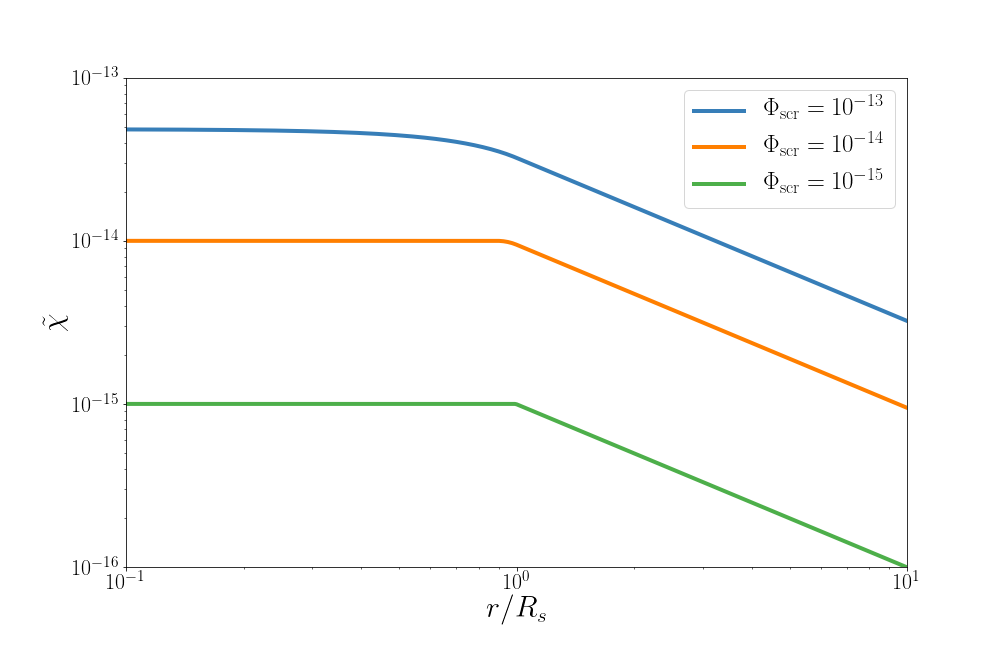
\includegraphics[width=1.0\linewidth]{{spherical_cham/starlike}.png}
	\caption{Chameleon profile for several screening potentials. The top solution is in the linear regime and is identical to the gravitainal potential. The other two solutions are in the screened regime and the amplitude of the field is suppressed.}
	\label{fig:starlike}
\end{figure}



In \autoref{fig:starlike_forces} \todo{describe forces}
\begin{figure}
	\centering
	
\includegraphics[width=1.0\linewidth]{{spherical_cham/starlike_forces}.png}
	\caption{Chameleon force relative to the standard gravitainal force for several screening potentials (given through the equivalence radius). For $R_{eq}\ll R_S$ there is no sreening outside the object. As the $R_{eq}$ grows the chameleon enters the screened regime.}
	\label{fig:starlike_forces}
\end{figure}

\subsubsection{NFW Halo}
In \autoref{fig:nfwlike_forces} \todo{describe forces}
\begin{figure}
	\centering
	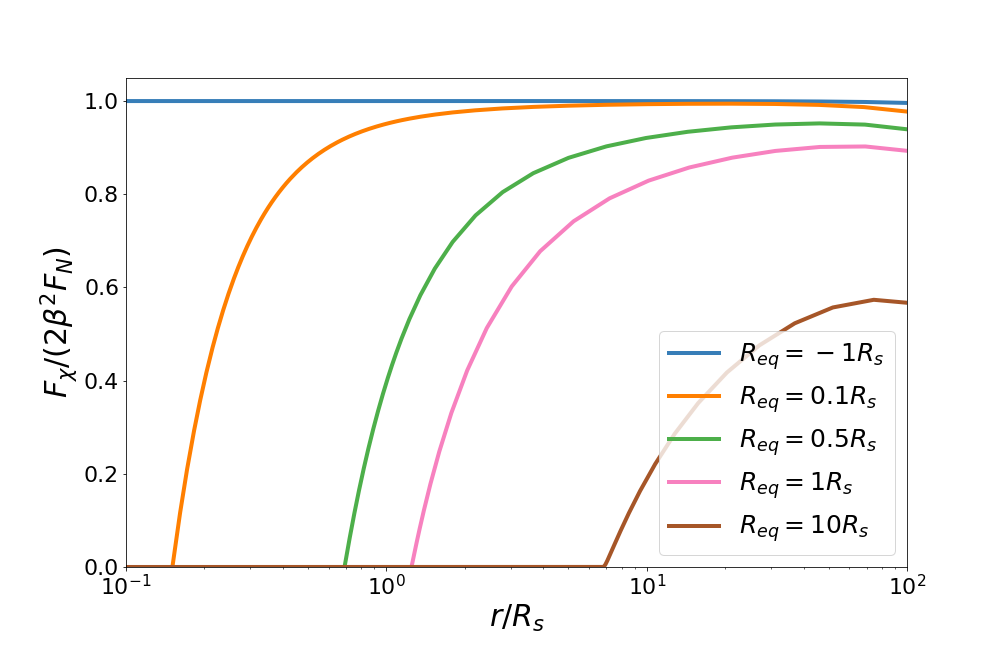
\includegraphics[width=1.0\linewidth]{{spherical_cham/nfwlike_forces}.png}
	\caption{Chameleon force relative to the standard gravitainal force for several screening potentials (given through the equivalence radius). For $R_{eq}\ll R_S$ there is no sreening outside the object. As the $R_{eq}$ grows the chameleon enters the screened regime.}
	\label{fig:nfwlike_forces}
\end{figure}


In \autoref{fig:nfwlike_pot_eff} \todo{describe effective screening potential}

\begin{figure*}
	\centering
		\begin{subfigure}{1.0\linewidth}
			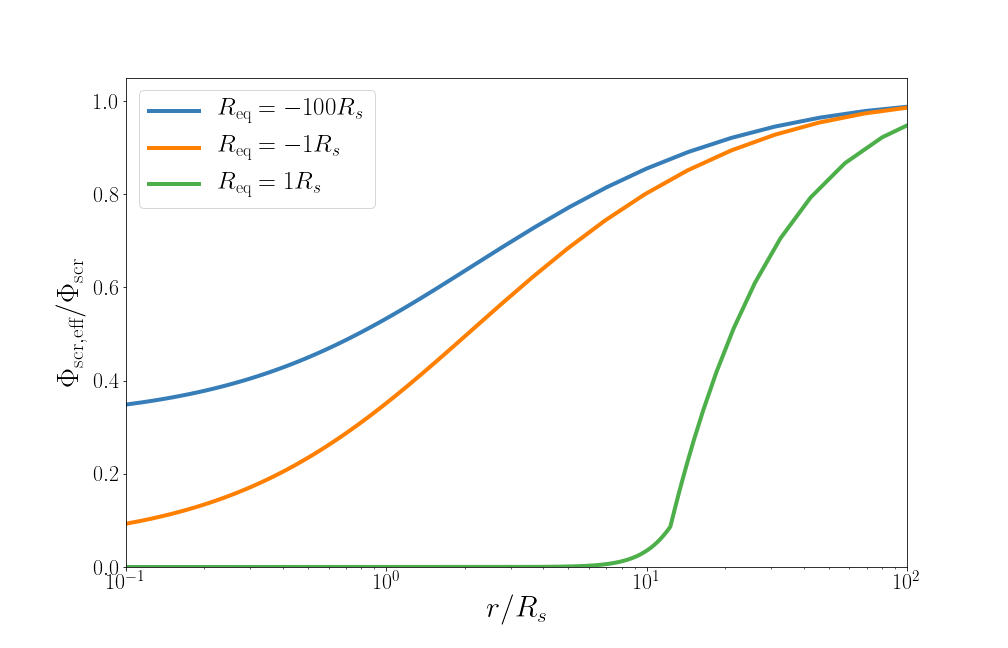
\includegraphics[width=1.0\linewidth]{{spherical_cham/nfwlike_pot_eff}.png}
		\end{subfigure}
		\begin{subfigure}{1.0\linewidth}
			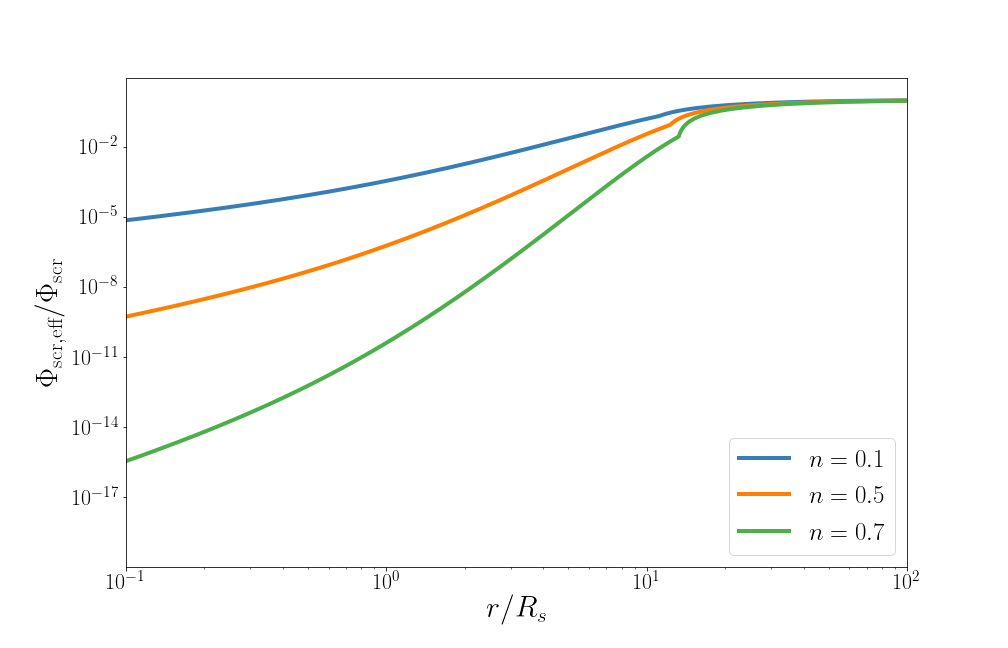
\includegraphics[width=1.0\linewidth]{{spherical_cham/nfwlike_pot_eff_n}.png}
		\end{subfigure}
		\caption{Effective screening potential relative to the screening potential for a cluster of galaxy, $M=10^{14} M_\odot, c=4$. Top Figure is shown for several screening potentials (given through the equivalence radius) while the bottom for different chameleon parameter $n$.}
		\label{fig:nfwlike_pot_eff}
\end{figure*}

In \autoref{fig:clustersYs} \todo{describe dynamical and lensing measurements}
\begin{figure*}
\begin{adjustwidth}{-3cm}{-1cm}
	\centering
		\begin{subfigure}{0.5\linewidth}
			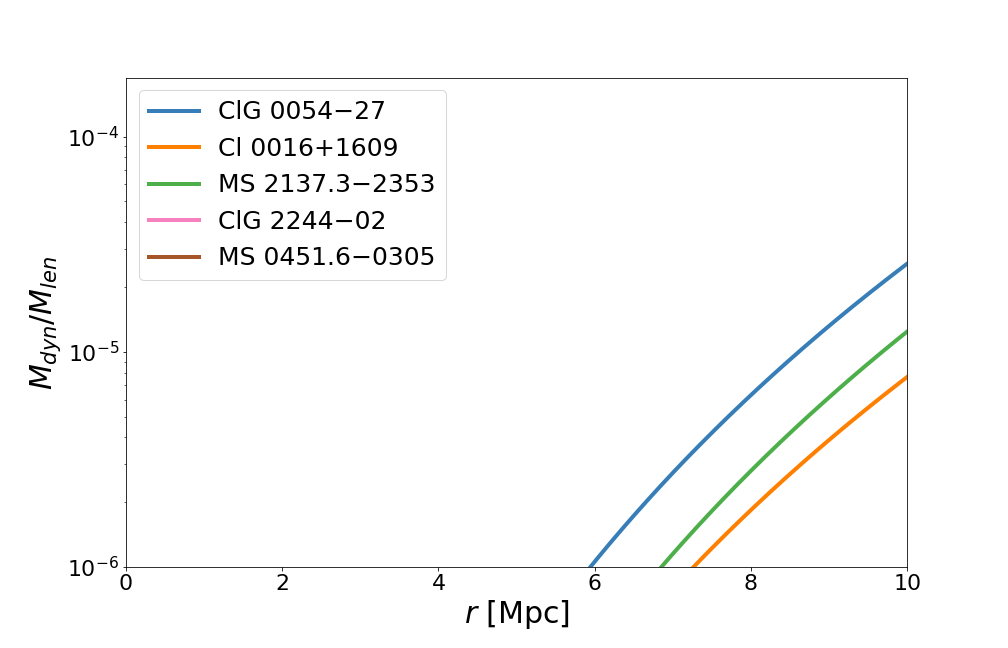
\includegraphics[width=1.0\linewidth]{{spherical_cham/clustersYs_-6}.png}
			\caption{$\Phiscr=10^{-6}$}
		\end{subfigure}%
		\begin{subfigure}{0.5\linewidth}
			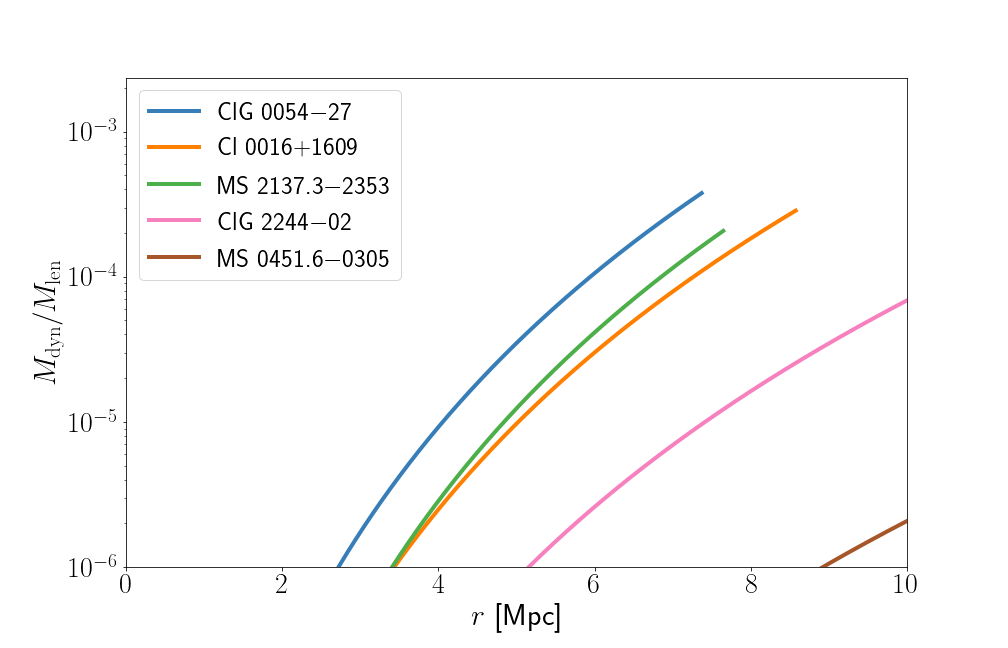
\includegraphics[width=1.0\linewidth]{{spherical_cham/clustersYs_-4}.png}
			\caption{$\Phiscr=10^{-4}$}
		\end{subfigure}
		\begin{subfigure}{0.5\linewidth}
			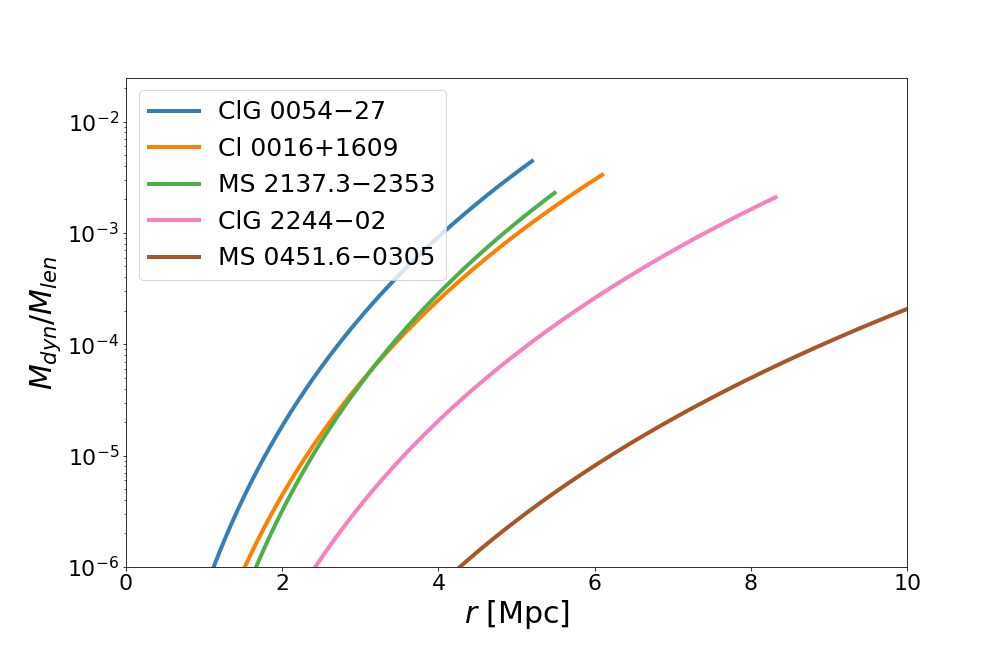
\includegraphics[width=1.0\linewidth]{{spherical_cham/clustersYs_-2}.png}
			\caption{$\Phiscr=10^{-2}$}
		\end{subfigure}%
		\begin{subfigure}{0.5\linewidth}
			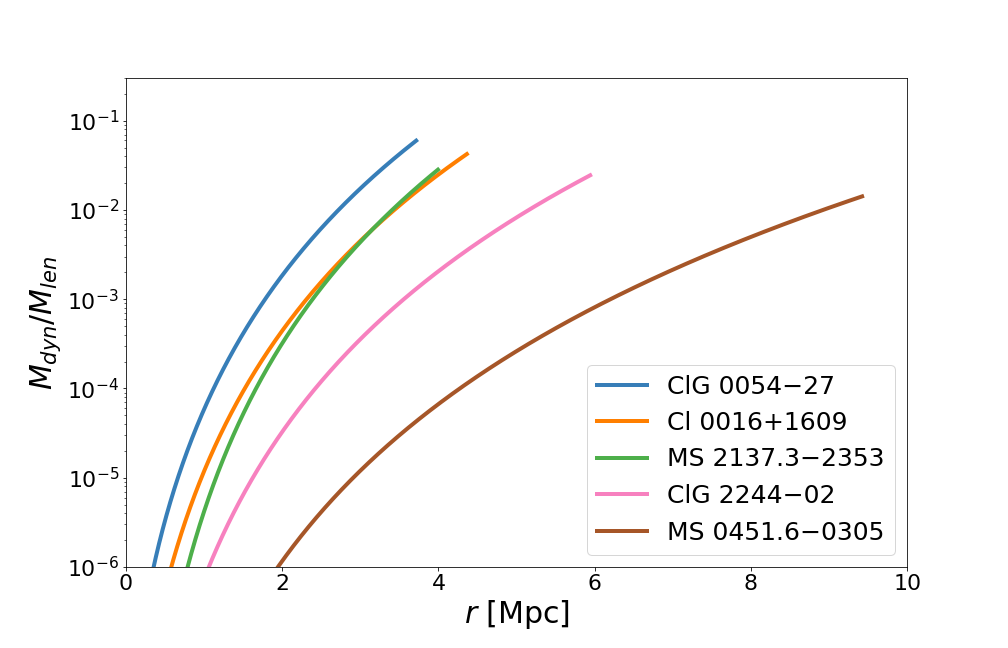
\includegraphics[width=1.0\linewidth]{{spherical_cham/clustersYs_0}.png}
			\caption{$\Phiscr=10^{0}$}
		\end{subfigure}
		\caption{Effective dynamical mass of the clusters relative to the actual (lensing) mass of the cluster. Cluster properties are: ClG 0054-27 $(c=1.2, M=0.42\cdot10^{14}M_\odot)$, Cl 0016+1609 $(c=2.1, M=1.12\cdot10^{14}M_\odot)$, MS 2137.3-2353 $(c=13, M=2.9\cdot10^{14}M_\odot)$, ClG 2244-02 $(c=4.3, M=4.5\cdot10^{14}M_\odot)$, MS 0451.6-0305 $(c=5.5, M=18\cdot10^{14}M_\odot)$. Parameters are taken from \textcite{2007MNRAS.379..190C}.}
		\label{fig:clustersYs}
\end{adjustwidth}
\end{figure*}